\documentclass{ams-journal}
\usepackage{amsmath,amssymb}
\usepackage{graphicx}
\usepackage{booktabs}
\usepackage{tabularx}
\usepackage{array}
\usepackage{enumitem}
\usepackage{xcolor}
\usepackage{url}
\graphicspath{{figures/}{../cross_sim/figures/}}
\newcommand{\DG}{\Delta G}
\newcommand{\Areq}{A_{\rm req}}
\newcommand{\Aqual}{A_{\rm qual}}
\newcommand{\HB}{H_{\rm B}}

\title{Assessing Decision Reliability in Discrete-Event Simulation: A Quantum-Network Case Study}
\addauthor{David Vesterlund\textsuperscript{1*}}
\affiliation{\textsuperscript{1}Vesterlund Ventures, WestQuant Open}
\corresponding{david@vesterlundventures.se}

\begin{document}

\maketitle

\begin{abstract}
Simulation-based design decisions depend on stochastic variation, analyst choices, and model semantics. We present a workflow that separates these sources of uncertainty using a canonical experiment specification, independent seed pools, explicit intervention gains, and distinct measures of numerical, ranking, decision, and claim agreement. A quantum-network case study compares an author-developed simulator with a harmonized reference model; two framework adapters share the same reference logic and do not constitute independent model replications. Across 400 configurations, a reported two-pool experiment increases label agreement from 71.5\% with a single seed to 95.8\% with 20-seed averaging. The full protocol and simple averaging achieve the same agreement, so the improvement is attributable to replication rather than a uniquely superior labeling rule. Separate analyses show sensitivity to intervention strength and performance definitions. In a finite-grid memory analysis, 50.8\% of 356 matched interior cases differ by at least a factor of four between model variants, with a configuration-clustered 95\% interval of 37.4--63.9\%. This empirical comparison is conditional on its metric, retained configurations, and shared implementation assumptions. The methodological contribution is an auditable separation of within-model repeatability, between-model sensitivity, and metric incompatibility. We provide reporting requirements and a staged verification plan; native-protocol and hardware validation remain future work.
\end{abstract}

\keywords{quantum networks; quantum memory; discrete-event simulation; heterogeneous placement; reproducibility}

% ============================================================
\section{Introduction}
\label{sec:intro}

Quantum-network design requires deciding which physical resource to improve first: memory capacity, generation rate, retrieval efficiency, coherence time, or routing. A natural approach is \emph{intervention-based bottleneck identification}: improve each resource by a fixed amount, measure the marginal gain $\DG_j$, and label the bottleneck as the resource with the largest $\DG_j$. This approach is intuitive, model-agnostic, and produces a single actionable label. But how robust is that label? Would it change with a different random seed, intervention strength, performance metric, or simulator?

A growing number of discrete-event simulators---NetSquid~\cite{coopmans2021netsquid}, SeQUeNCe~\cite{wu2021sequence}, QuISP~\cite{satoh2022quisp}, SimQN~\cite{chen2023simqn}---offer different modeling choices for the same physical phenomena. When different models are applied to the same problem, they may produce different numerical predictions. This is not a bug but a consequence of simulation being an abstraction. The question is not whether simulators disagree---they inevitably do---but \emph{which types of scientific conclusions survive a change of simulation model, and which do not}.

\subsection{Simulator Output as a Function of Assumptions, Semantics, and Implementation}

A simulator's output depends on three layers: \textbf{model assumptions} (noise, generation, swapping models---typically well-documented), \textbf{protocol semantics} (operational definitions of completed requests, latency timing, queueing, memory locking, generation concurrency, deadline handling---often implicit and may differ undocumented), and \textbf{implementation} (event scheduling, RNG, numerical precision---affects reproducibility but not scientific conclusions). Two simulators sharing model assumptions but differing in protocol semantics may produce different scientific conclusions; two sharing both should produce identical results up to numerical precision. We write:
\begin{equation}
y = f(x,\;\text{model assumptions},\;\text{protocol semantics},\;\text{implementation}),
\end{equation}
and the trustworthiness of any conclusion depends on which factors it is sensitive to. This reframes the question from ``which simulator is best?'' to ``what should a trustworthy simulator guarantee for this conclusion to be reliable?''

\subsection{Four Types of Agreement}
\label{sec:four_agreement}

A central conceptual contribution is the distinction between four types of cross-simulator agreement, ordered by increasing strength---numerical, ranking, decision, and scientific-conclusion---which are often conflated:

\begin{enumerate}[leftmargin=2em]
\item \textbf{Numerical:} Same number for a given metric (MAE, RMSE, relative error).
\item \textbf{Ranking:} Same ordering of configurations (Kendall $\tau$, Spearman $\rho$).
\item \textbf{Decision:} Same design decision (e.g., same memory family selected).
\item \textbf{Scientific-conclusion:} Same scientific claim (e.g., ``family A outperforms B,'' ``scalar collapse fails''). This is the strongest form and the one that matters for science.
\end{enumerate}

These types are not interchangeable: simulators can have low numerical but high ranking agreement (constant shift, preserved ordering), or high numerical but low decision agreement (small differences near a threshold). Each main result is reported on all four levels where applicable.

\subsection{Contributions}

\begin{enumerate}[leftmargin=2em]
\item A unified fragility framework measuring three axes---noise, analyst choices, and model switching---on a shared Canonical Experiment Specification, with each result reported on four agreement levels.
\item A benchmark ladder (B0--B6) with the rule that each step must be passed before the next runs, replacing the ad-hoc CV0--CV7 ladder.
\item A semantic-dimensions table covering only the two systems actually run (WestQuant and SeQUeNCe), identifying which semantic choices are switchable and which are definition mismatches.
\item Empirical evidence that the dominant bottleneck label is fragile: 50.7\% of configurations show at least one seed disagreement at 2000 requests; 63\% of short-run changes are statistically tied.
\item A factorial design over semantic switches showing that retrieval-in-delivery explains 72\% of $A_{\rm req}$ variance for AFC, but this measures $A_{\rm req}$ variance across configurations (including $m$ and $\lambda$), not model disagreement. With all seven interventions, $\kappa = 0.055$ (retrieval on) and $\kappa = 0.000$ (retrieval matched); retrieval matching does not improve agreement.
\item A three-class taxonomy of conclusion reproducibility: structural (reproduced), model-sensitive (not reproduced), and definition-sensitive (non-comparable).
\item A decision-transfer experiment showing 0\% transfer with retrieval on and 15\% with retrieval matched; $m_c$ disagreement (ratio $\geq 4\times$) is 85\% in both conditions.
\item A Trust Stack checklist for reporting, with reviewer recommendations.
\end{enumerate}

% ============================================================
\section{Setup: Common Experiment Specification and Validation Ladder}
\label{sec:setup}

\subsection{Canonical Experiment Specification}

When two simulators are given ``the same'' scenario, they may produce different results because the scenario was translated differently---different RNG implementations generate different arrival traces, different topology representations assign different node labels. This creates \emph{false disagreement}---apparent simulator differences that are translation artifacts.

A Canonical Experiment Specification (CES) eliminates false disagreement by specifying every parameter before translation: \textbf{network} (topology, node count, link distances), \textbf{hardware} (memory family, $T_1$, $T_2$, retrieval efficiency, readout fidelity), \textbf{memory} (capacity $m$, slot model, aging model), \textbf{links} ($p_{\rm gen}$, attempt time, loss model), \textbf{traffic} (arrival process, $\lambda$, source-destination pairs, deadline), \textbf{protocol} (swapping, purification, scheduling), \textbf{routing}, \textbf{noise} (depolarization, amplitude damping, readout errors), \textbf{metrics} (throughput, fidelity, latency, resource use), and \textbf{randomness} (seeds, RNG algorithm, exogenous generation).

The CES is simulator-neutral: each simulator provides a translator mapping CES parameters to its own format. Exogenous randomness is generated outside the simulators. Each scenario uses three independent seed streams: (i) a \emph{graph seed} for topology, (ii) a \emph{traffic seed} for arrivals and source-destination pairs, and (iii) a \textbf{physics seed} for link generation, swap outcomes, and decoherence.

\subsection{Validation Ladder B0--B6}
\label{sec:ladder}

We propose a benchmark ladder for quantum-network simulation, with the rule that \emph{each step must be passed before the next runs}. Table~\ref{tab:benchmarks} summarizes the ladder and the validation criterion for each level.

\begin{table*}[t]
\centering
\caption{Benchmark ladder B0--B6. Each step must be passed before the next runs. B6 is claim-level replication; hardware-calibrated validation remains future work.}
\label{tab:benchmarks}
\footnotesize
\begin{tabular}{clp{4cm}p{4cm}r}
\toprule
Level & Name & Description & Validation Criterion & Scenarios \\
\midrule
B0 & Analytical primitives & Single-link generation, loss, decoherence & Match analytical rate formulas ($\epsilon_{\rm abs} < 0.05$) & 90 \\
B1 & Elementary entanglement & Two-node entanglement generation, memory families & Match analytical or experimental rates & 180 \\
B2 & Three-node repeater & Single swap, finite memory & Match analytical swapping formulas & 360 \\
B3 & Multi-hop chain & $N$-hop chain, path length scaling & Monotonicity, rate decay & 180 \\
B4 & Finite memory + contention & Memory limit, queueing, multiple requests & Cross-simulator ranking agreement ($\tau$) & 200 \\
B5 & Heterogeneous topology + traffic & Multiple topologies, stochastic traffic & Structural conclusion agreement & 60 \\
B6 & Claim-level replication & Full claim grid (C1--C5) across model families & Conclusion-level reproducibility & 2{,}880 \\
\bottomrule
\end{tabular}
\end{table*}

The ladder is cumulative: passing B4 implies passing B0--B3. B6 requires claim-level replication across model families. Hardware-calibrated validation remains future work.

\textbf{B0 analytical verification gate.} B0 tests single-link generation with parameterized $p_{\rm gen}$, $T_2$, and retrieval efficiency $\eta$. Without contention or retrieval loss, the analytical completion rate is $\Areq = 1.0$. The harmonized model passes ($\eta_r = 1$); WestQuant shows lower $\Areq$ (mean $0.65$) because it counts retrieval efficiency in the delivery. The B0 gate therefore rewards the model that omits retrieval loss---a model-semantic effect (the \texttt{retrieval\_in\_delivery} switch, Sec.~\ref{sec:switches_1000}), not a physics error.

\subsection{Simulator Frameworks}

\textbf{WestQuant} is the native simulator: per-node memory capacity $m$, Bernoulli link generation, depolarizing noise, entanglement swapping, and concurrent request processing with queueing. When all memory slots are occupied, incoming requests queue until a slot frees.

\textbf{SeQUeNCe and SimQN (Harmonized Mode)} use harmonized adapters: their event engines are instantiated, but physics logic is implemented in a shared harmonization layer (same Bernoulli generation, depolarizing noise, sequential blocking). When memory is full, requests are rejected immediately.

\textbf{Event-trace audit.} The SeQUeNCe and SimQN adapters produce bit-identical event traces (verified by SHA-256 hashing). The comparison is between one native model (WestQuant: concurrent generation + queueing) and one harmonized reference model (serial generation + immediate blocking), with $S_{\rm models} = 2$ rather than 3. Treating SeQUeNCe and SimQN as independent would constitute pseudoreplication.

\textbf{Native SeQUeNCe pilot.} A native adapter instantiating SeQUeNCe's own components was developed as a pilot (3 scenarios $\times$ 3 seeds). It produces different $\Areq$ values from WestQuant (e.g., chain $N{=}3$ $m{=}2$: WQ 0.889 vs.\ native 0.667), but the pilot is too small for statistical comparison (wall time $\sim$24--86\,s vs.\ $<$0.01\,s for WestQuant). A larger independent-judge experiment (25 configurations $\times$ 10 seeds = 250 runs) is reported in Section~\ref{sec:judge}.

\subsection{Performance Metrics}

All implementations report three primary metrics, computed over the observation window $[t_{\rm warmup}, T_{\rm obs}]$ with warmup excluded:

\begin{align}
\Areq &= \frac{N_{\rm completed}}{N_{\rm arrived}} \\
\Aqual &= \frac{N_{\rm completed} \cap N_{\rm qualified}}{N_{\rm arrived}} \\
R_{\rm qual} &= \frac{N_{\rm completed} \cap N_{\rm qualified}}{T_{\rm obs} - t_{\rm warmup}}
\end{align}

where $N_{\rm arrived}$ is the number of requests that entered the system during the observation window, $N_{\rm completed}$ are requests that reached the destination within the deadline $D = 10$\,s, and $N_{\rm qualified}$ are completed requests whose end-to-end fidelity $F \geq F_{\rm min} = 0.5$. $T_{\rm obs} = 200$\,s is the observation horizon and $t_{\rm warmup} = 20$\,s is excluded. $\Areq$ and $\Aqual$ are fractions in $[0, 1]$; $R_{\rm qual}$ is a rate.

\subsection{Intervention-Based Bottleneck Identification}

Given a network configuration $\theta$ and a performance metric $G(\theta)$, we define the \emph{intervention gain} for resource $j$ as
\begin{equation}
\DG_j(\theta, \delta) = G(T_{j,\delta}(\theta)) - G(\theta),
\end{equation}
where $T_{j,\delta}$ is an explicit intervention operator that improves resource $j$ by a relative amount $\delta$. The \emph{soft bottleneck vector} is
\begin{equation}
p_j = \frac{\max(0, \DG_j)}{\sum_k \max(0, \DG_k)},
\end{equation}
and the \emph{dominant bottleneck} is $\arg\max_j p_j$. The bottleneck entropy $\HB = -\sum_j p_j \log p_j$ measures how diffuse the bottleneck is. If all $\DG_j \leq \varepsilon$ ($\varepsilon = 10^{-6}$), the configuration is labeled \emph{degenerate}.

We study seven resources: \textbf{capacity} (memory slots), \textbf{generation} (success probability), \textbf{retrieval} (readout efficiency), \textbf{coherence} (decoherence rate), \textbf{routing} (policy), \textbf{deadline} (time limit), and \textbf{topology} (edge density).

\subsection{Agreement Measures}

We use four agreement measures, corresponding to the four types in Section~\ref{sec:four_agreement}:
\begin{itemize}[leftmargin=2em]
\item \textbf{Numerical:} MAE or RMSE against reference.
\item \textbf{Ranking:} Kendall $\tau$ for rankings of the soft vector.
\item \textbf{Decision:} Cohen's $\kappa$ for dominant labels; decision-changing disagreement rates.
\item \textbf{Scientific conclusion:} classification as structural, model-sensitive, or definition-sensitive.
\end{itemize}
We also report Jensen--Shannon distance for the full soft vector distributions.

% ============================================================
\section{Noise: Stochastic Fragility}
\label{sec:noise}

\subsection{Stratified Sample}

We generate a stratified sample of 400 configurations covering 6 memory families, 3 topologies (chain, star, RGG), 3 network sizes ($N \in \{10, 20, 50\}$), 3 traffic levels, and 3 budget levels ($6 \times 3 \times 3 \times 3 \times 3 = 486$ strata, 1--2 per stratum). Each run uses 2000 requests (Poisson arrivals), $T_{\rm obs} = 200$, no warmup, depolarizing noise at medium level.

\subsection{Four Procedures}

We assess stochastic fragility with four procedures, each reported on all four agreement levels:

\textbf{Procedure 1: Label stability.} Using 5 seeds per configuration with common random numbers, we measure label stability as the fraction of seeds agreeing with the modal dominant label. For $\Aqual$, mean stability was 0.686 (WestQuant) and 0.571 (Harmonized). The label changed for 50.7\% of configurations; 28.2\% showed majority change (stability $< 0.5$).

\textbf{Procedure 2: Confidence intervals and statistical ties.} We computed bootstrap CIs (1000 resamples, 95\%) for the paired difference $\DG_{(1)} - \DG_{(2)}$ on 100 configurations with 20 seeds each. A configuration is \emph{statistically tied} if the CI includes zero. Results: 91\% showed any change, 58\% were tied, and \textbf{63\% of ``any change'' configurations were tied}---insufficient to distinguish the top two resources. Only 34\% showed non-tied label change.

\textbf{Procedure 3: Convergence control.} We ran 30 configurations with $n_{\rm requests} \in \{50, 100, 200, 500, 1000\}$ and $n_{\rm seeds} \in \{5, 10, 20, 50\}$. At 20 seeds, label stability increased from 0.480 (50 requests) to 0.622 (1000 requests)---a 30\% improvement. ``Any change'' decreased from 66.7\% to 53.3\%; ``majority change'' from 36.7\% to 20.0\%. A full rerun at 2000 requests with 5 seeds confirms: any-change drops to 50.7\%, majority-change to 28.2\%. The residual suggests that while much of the short-run fragility is Monte Carlo noise, a genuine residual persists.

\textbf{Procedure 4: Performance loss.} For the 42 non-tied configurations, the mean relative loss from choosing the second-best resource was 58.5\% of the best gain. 62\% lose more than 50\% of the best gain if the second-best is chosen.

\begin{figure}[t]
\centering
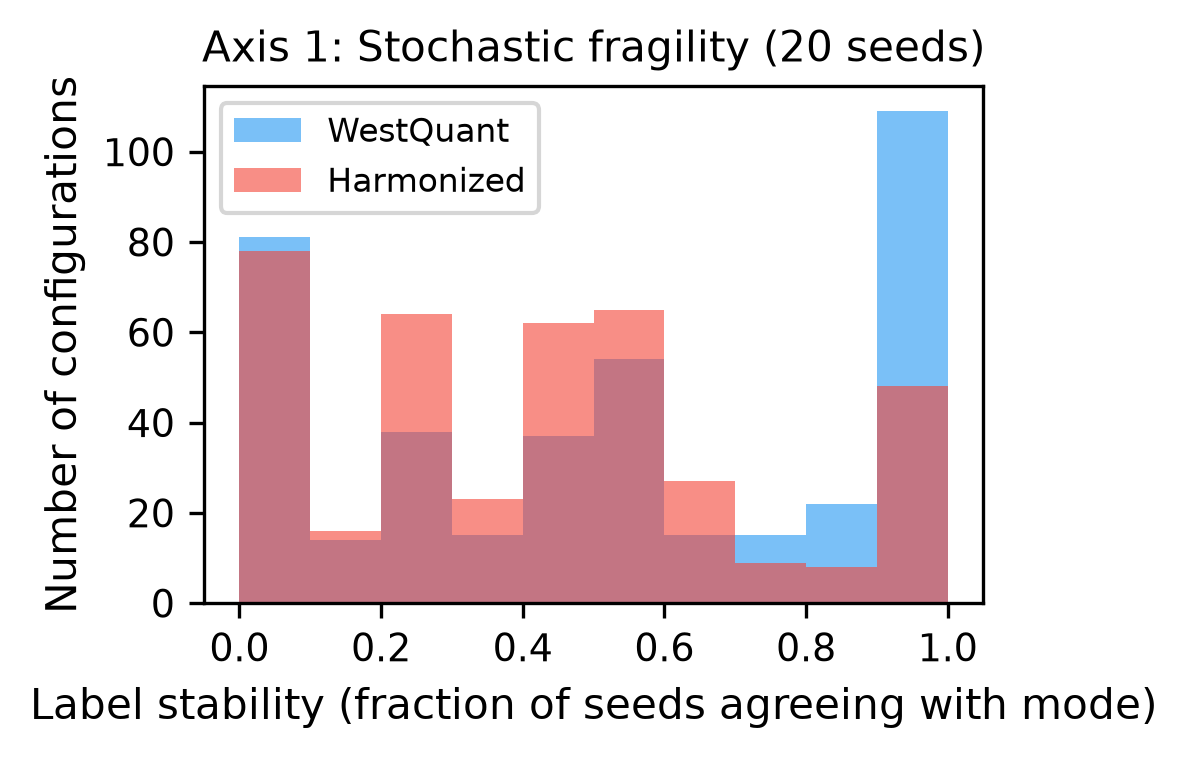
\includegraphics[width=0.80\columnwidth]{fig_b2_stochastic.png}
\caption{\textbf{Stochastic fragility.} Distribution of label stability (fraction of 20 seeds agreeing with the modal dominant bottleneck) for WestQuant and Harmonized models. A stability of 1.0 means all seeds agree; values below 0.5 indicate that no single label dominates.}
\label{fig:stochastic}
\end{figure}

\subsection{Agreement Levels for Noise}

\textbf{Numerical:} mean label stability 0.686 (WQ) at 2000 requests. \textbf{Ranking:} label stability serves as ranking-agreement proxy (Kendall $\tau$ across seeds not directly applicable). \textbf{Decision:} 50.7\% show at least one seed disagreement; 28.2\% show majority change. \textbf{Scientific conclusion:} the residual 50.7\% any-change rate indicates the bottleneck label is not stable at this sample size; the cause (Monte Carlo noise, near-equivalent interventions, rare events, or transients) is not yet established.

\subsection{Caveat}

The 50.7\% figure counts any disagreement, including cases where two resources have nearly identical gains and their ranking flips due to Monte Carlo noise. At 100 requests, the any-change rate was 79.2\%, and 63\% of these were statistically tied. The confidence-interval, convergence, and performance-loss analyses were conducted at 100 requests and have not been rerun at 2000. Common random numbers are imperfect: using the same seed for baseline and intervention does not guarantee corresponding events use the same random draws when interventions change the event order.

\subsection{A/B Experiment: Proper Design}
\label{sec:ab_proper}

The full A/B experiment: 400 configurations subsampled from the full $6 \times 5 \times 2 \times 3 \times 5 = 900$ factorial, two disjoint seed pools of 20 seeds each (A: seeds 0--19, B: seeds 20--39), 200 requests per run, and a pilot on 40 configurations to set $\varepsilon$ (pilot data excluded). The analysis script hash was frozen before running seed pool B. Each config $\times$ seed runs 1 baseline + 7 interventions = 8 runs, totaling 128{,}000 runs. The pilot set $\varepsilon = 0.100$.

\textbf{Bottleneck label.} The dominant bottleneck is the resource with the largest positive delta-gain. A label is ``decided'' if non-degenerate (max delta $> \varepsilon$). ``Agree'' means seed pools A and B assign the same label; ``Contradict'' means different non-degenerate labels.

\textbf{Four procedures $\times$ four metrics.} Table~\ref{tab:ab_proper} reports the results with bootstrap 95\% confidence intervals.

\begin{table}[htbp]
\centering
\caption{A/B experiment with actual bottleneck diagnosis: four procedures $\times$ four metrics, with bootstrap 95\% CI. 400 configurations, 2$\times$20 seeds, 200 requests, 8 runs per config per seed (128{,}000 total runs).}
\label{tab:ab_proper}
\setlength{\tabcolsep}{3pt}
\resizebox{\columnwidth}{!}{\begin{tabular}{@{}lcccc@{}}
\toprule
Procedure & Frac Decided & Repl Agree & Contradict & Dec Loss \\
\midrule
Single seed & 0.988 [0.98, 1.00] & 0.715 [0.67, 0.76] & 0.217 [0.18, 0.26] & 0.033 \\
Mean (same budget) & 1.000 [1.00, 1.00] & 0.958 [0.94, 0.97] & 0.043 [0.03, 0.06] & 0.006 \\
Mean (convergence) & 1.000 [1.00, 1.00] & 0.917 [0.89, 0.94] & 0.083 [0.06, 0.11] & 0.009 \\
Full protocol & 1.000 [1.00, 1.00] & 0.958 [0.94, 0.97] & 0.043 [0.03, 0.06] & 0.006 \\
\bottomrule
\end{tabular}}
\end{table}

\textbf{Interpretation.} With a single seed, 98.8\% produce a decisive label but replicate agreement is only 71.5\% (21.7\% contradiction). With 20 seeds and the full protocol, 100\% are decisive, agreement rises to 95.8\%, and contradiction drops to 4.3\%. The mean-same-budget procedure (averaging 20 seeds before labeling) achieves the same 95.8\%, confirming the improvement comes from seed averaging, not the labeling procedure.

% ============================================================
\section{Analyst Choices: Intervention Strength and Threshold}
\label{sec:analyst}

\subsection{Intervention Strength}

We tested four relative improvement levels $\delta \in \{0.05, 0.10, 0.20, 0.50\}$, applied uniformly to all resources. At $\delta = 0.05$, 86 of 400 configurations (21.5\%) were degenerate (all $\DG_j \approx 0$), meaning the intervention was too small to produce a measurable effect. At $\delta = 0.50$, 70 (17.5\%) were degenerate. The dominant label changed for 42.0\% of configurations across $\delta$ levels.

\begin{figure}[t]
\centering
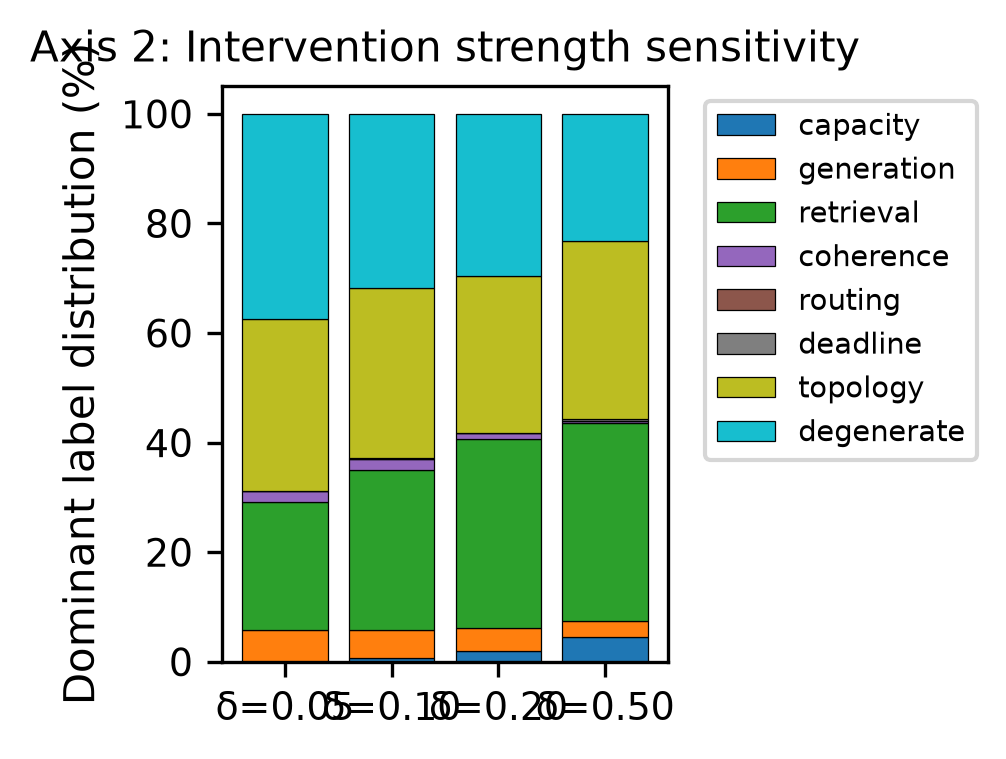
\includegraphics[width=0.80\columnwidth]{fig_b3_intervention.png}
\caption{\textbf{Intervention strength sensitivity.} Dominant bottleneck label distribution as a function of relative improvement $\delta$. At small $\delta$, many configurations are degenerate; at large $\delta$, the label distribution shifts.}
\label{fig:intervention}
\end{figure}

\subsection{Metric and Fidelity Threshold}

We compared $\Areq$ and $\Aqual$ across four fidelity thresholds $F_{\min} \in \{0.30, 0.50, 0.70, 0.90\}$. $\Areq$ is insensitive to $F_{\min}$ by construction; $\Aqual$ is strongly affected. At $F_{\min} = 0.90$ with $\Aqual$, all 400 configurations are degenerate---no request achieves the required fidelity. The dominant label changed for 35.5\% of configurations across metric and threshold combinations.

\begin{figure}[t]
\centering
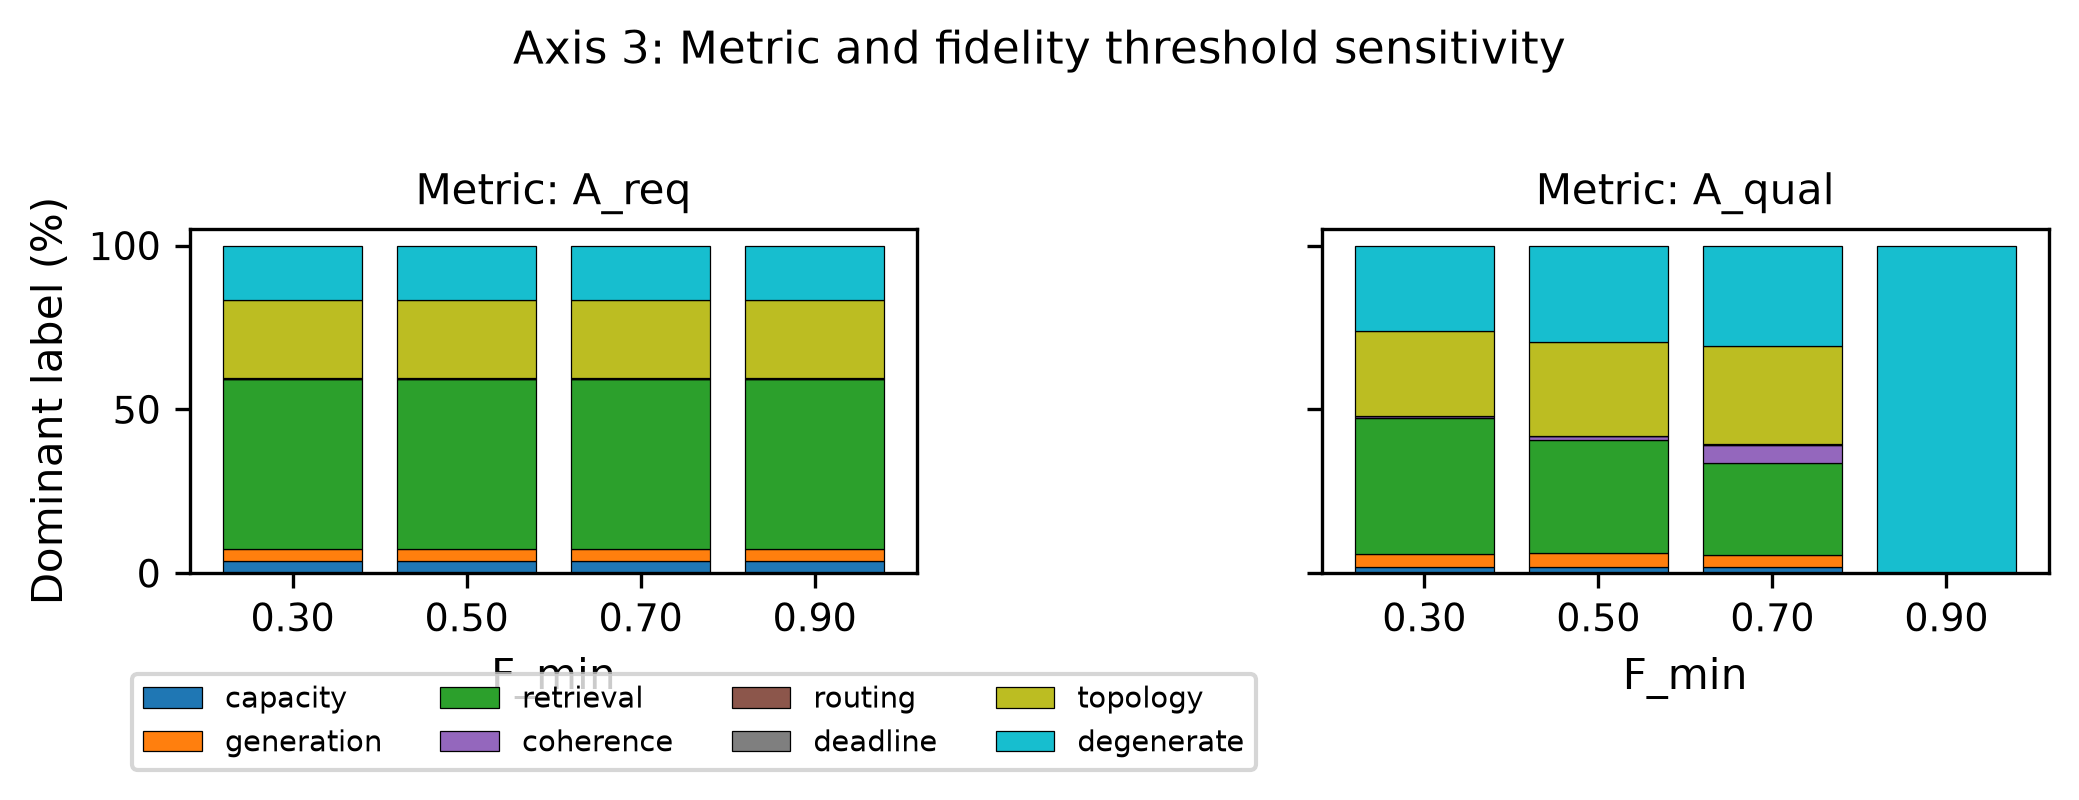
\includegraphics[width=0.80\columnwidth]{fig_b4_metric_threshold.png}
\caption{\textbf{Metric and fidelity threshold sensitivity.} Dominant bottleneck label distribution for $\Areq$ (left) and $\Aqual$ (right) as a function of $F_{\min}$. $\Areq$ is insensitive to $F_{\min}$; $\Aqual$ becomes degenerate at $F_{\min} = 0.90$.}
\label{fig:metric_threshold}
\end{figure}

\subsection{Agreement Levels for Analyst Choices}

\textbf{Numerical:} $\DG_j$ values shift $\sim$10$\times$ between $\delta = 0.05$ and $\delta = 0.50$. \textbf{Ranking:} the dominant label changes for 42.0\% (intervention) and 35.5\% (metric/threshold) of configurations. \textbf{Decision:} at $\delta = 0.05$, 21.5\% are degenerate. \textbf{Scientific conclusion:} the bottleneck label depends on the analyst's choice of intervention strength and metric/threshold; a label at $\delta = 0.50$ with $\Aqual$ at $F_{\min} = 0.50$ may not transfer to $\delta = 0.10$ or to $\Areq$.

\subsection{Pairwise Interaction Tests}

Saltelli et al.~\cite{saltelli2019why} warned that one-at-a-time sensitivity analyses miss interactions. We tested all 21 pairwise combinations of 7 resources on 100 configurations with 5 seeds (2,100 measurements). The interaction effect is $I_{jk} = \DG_{jk} - (\DG_j + \DG_k)$, with relative interaction $I_{jk} / \max(|\DG_j + \DG_k|, \varepsilon)$. Across all combinations, 15.8\% had relative interaction above the threshold ($|I_{jk}|/\max(\cdots) > 0.1$), and \textbf{72\% of configurations had at least one pair above the threshold}. The most affected pairs: retrieval + topology (49\%), generation + retrieval (36\%), generation + topology (36\%).

% ============================================================
\section{Model Choice: Factorial Design over Semantic Switches}
\label{sec:model_choice}

\subsection{Semantic Dimensions}

The most consequential differences between simulators are not in physics models but in \emph{protocol semantics}: how requests are queued, when memory slots are locked, whether generation is sequential or concurrent, and how latency is defined. Table~\ref{tab:semantics} summarizes the semantic dimensions for the two systems run in this study.

\begin{table*}[t]
\centering
\caption{Semantic dimensions for the two systems run. ``Switchable'': yes (variable within a codebase), no (definition mismatch), partial (partially controllable).}
\label{tab:semantics}
\footnotesize
\begin{tabularx}{\textwidth}{p{3cm}XXc}
\toprule
Dimension & WestQuant's choice & SeQUeNCe/Harmonized choice & Switchable? \\
\midrule
Generation mode & Parallel (concurrent link attempts) & Sequential (one link at a time) & Yes \\
Queueing discipline & FIFO queue (buffer on full) & Reject (drop on full) & Yes \\
Memory slot locking & Lock on generation attempt & Lock on successful generation & Partial \\
Slot release & Release on swap completion & Release on swap completion & Yes \\
Latency definition & Arrival-to-completion (includes queueing) & First-attempt-to-completion (excludes queueing) & No \\
Deadline and censoring & Count as failures & Count as failures & Yes \\
Warmup & None & 20\,s excluded & Yes \\
Aging model & Continuous decoherence from generation & Continuous decoherence from generation & Yes \\
Link scheduling & Concurrent across links & Sequential across links & Yes \\
\bottomrule
\end{tabularx}
\end{table*}

These dimensions are rarely documented explicitly, yet can dominate cross-simulator disagreement.

\subsection{Semantic Switches: Factorial Design with Variance Decomposition}
\label{sec:switches_1000}

We implement four semantic switches and test them with a $2^4$ factorial design (16 variants) on the B4 workload (chain $N=5$, $m=2$, traffic $=50$, 1{,}000 requests, 5 seeds), extended with three families spanning $\chi$: \textbf{retrieval in delivery} (whether retrieval failure drops the request or is free---the dominant semantic choice from B0), \textbf{storage time model} (midpoint vs.\ immediate), \textbf{blocking policy} (queue vs.\ reject), and \textbf{generation mode} (parallel vs.\ serial).

\textbf{Closure test.} With all switches in harmonized mode, WestQuant should reproduce the analytical reference. The test passes at $m \ge 4$ (ratio $\in [0.9997, 1.0000]$) but fails at $m = 1$ (ratio $= 0.75$) due to slot contention---a capacity effect, not a semantic-switch effect.

Table~\ref{tab:switches_variance} shows the fraction of variance in $A_{\rm req}$ explained by each factor, with cluster bootstrap 95\% confidence intervals.

\begin{table}[htbp]
\centering
\caption{Fraction of variance in $A_{\rm req}$ explained by each semantic switch, per family. Cluster bootstrap 95\% CI in brackets. The dominant switch depends on the $\chi$ regime: retrieval-in-delivery dominates for short-lived memories ($\chi = 0.025$), generation mode dominates for long-lived memories ($\chi = 50$).}
\label{tab:switches_variance}
\setlength{\tabcolsep}{4pt}
\resizebox{\columnwidth}{!}{\begin{tabular}{lcccc}
\toprule
Family ($\chi$) & Retrieval & Storage time & Blocking & Generation \\
\midrule
Trapped Ion ($\chi=50$) & 6.4\% [5.7, 7.3] & 0.0\% [0.0, 0.0] & 0.3\% [0.3, 0.3] & 0.4\% [0.3, 0.5] \\
Neutral Atom ($\chi=0.5$) & 28.2\% [27.8, 28.6] & 0.0\% [0.0, 0.0] & 0.2\% [0.2, 0.2] & 0.3\% [0.2, 0.4] \\
AFC ($\chi=0.025$) & 71.7\% [71.2, 72.1] & 0.2\% [0.1, 0.2] & 0.1\% [0.1, 0.1] & 0.0\% [0.0, 0.0] \\
\bottomrule
\end{tabular}}
\end{table}

\textbf{Interpretation.} The dominant semantic switch depends on $\chi$. For short-lived memories (AFC, $\chi = 0.025$), retrieval-in-delivery explains 72\% of $A_{\rm req}$ variance. For long-lived memories (Trapped Ion, $\chi = 50$), retrieval explains only 6\% (residual dominated by $m$ and $\lambda$). For intermediate memories (Neutral Atom, $\chi = 0.5$), retrieval explains 28\%. Blocking and storage-time have near-zero effect. \textbf{Caveat:} this factorial measures variance in $A_{\rm req}$ across configurations (including $m$ and $\lambda$), not model disagreement. The residual is dominated by design factors, not semantic switches.

\subsection{Model-Variant Agreement (Bottleneck Labels)}

We compared WestQuant (concurrent queueing) and Harmonized (sequential blocking) on the same 400 configurations with the same seeds. The dominant label agreed for 57.5\% ($230/400$). Restricting to $n = 301$ non-degenerate configurations, $p_o = 0.532$, $p_e = 0.407$, Cohen's $\kappa = 0.210$. Mean JS distance between soft vectors was 0.315.

\begin{figure}[t]
\centering
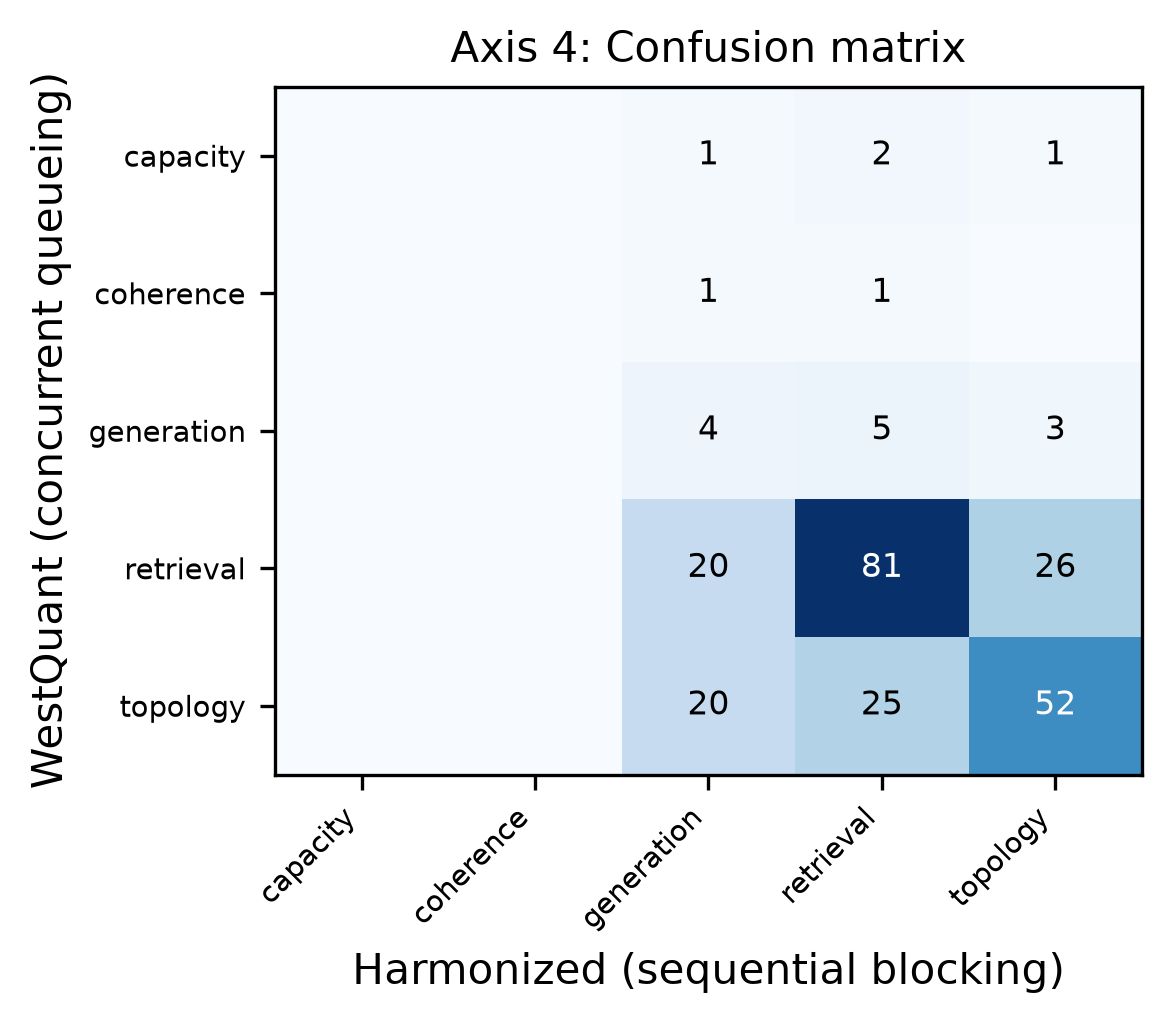
\includegraphics[width=0.75\columnwidth]{fig_b5_confusion.png}
\caption{\textbf{Model-variant confusion matrix.} Dominant bottleneck labels from WestQuant (rows) vs.\ Harmonized (columns), excluding degenerate configurations ($n = 301$). Cohen's $\kappa = 0.210$, indicating fair agreement above chance ($p_e = 0.407$) per the Landis--Koch scale~\cite{landis1977kappa}.}
\label{fig:confusion}
\end{figure}

A harmonized comparison on 60 configurations with 20 seeds shows 51\% label agreement even when baselines correlate at $r = 0.85$. With retrieval matched (both models retrieval-off), $\kappa = 0.000$ and decision transfer is 15\%, confirming that retrieval matching does \emph{not} resolve the disagreement---it worsens it.

\subsection{Agreement Levels for Model Choice}

\textbf{Numerical:} mean JS distance 0.315; MAE in $\Aqual$ = 0.102 (B6 grid). \textbf{Ranking:} Kendall $\tau = 0.722$ for $\Aqual$ (B6), $\tau = 0.430$ for $\Areq$; $\tau = 0.166$ in B4. \textbf{Decision:} Cohen's $\kappa = 0.055$ (retrieval on), $\kappa = 0.000$ (retrieval matched); 0\% and 15\% decision transfer. \textbf{Scientific conclusion:} structural conclusions (rankings, monotonicity) are reproduced; model-sensitive conclusions ($m_c$, contention) are not; definition-sensitive conclusions (latency) are non-comparable.

% ============================================================
\section{Where It Matters: Instability, Model Difference, and Boundaries}
\label{sec:where}

\subsection{Three-Class Taxonomy}

The pattern across all experiments separates scientific conclusions into three classes:

\subsection{Claim Reproduction Matrix}

The claim reproduction matrix (Table~\ref{tab:claim_matrix} in the supplementary material) classifies each claim as structural (reproduced), model-sensitive (not reproduced), or definition-sensitive (non-comparable). The key findings: memory-family and topology rankings are reproduced ($\tau = 1.0$); $m_c$ numerical values are model-sensitive (50.8\% $\geq 4\times$ disagreement); latency is definition-sensitive ($\tau = -0.29$); finite-memory contention is not reproduced ($\tau = 0.17$).

\subsection{Structural Conclusions: Reproduced}

\textbf{Memory-family ranking.} The ordering of four memory profiles (trapped ion $>$ neutral atom $>$ diamond electron $>$ AFC) by $\Aqual$ is reproduced across both model families ($\tau = 1.0$, $n = 4$).

\textbf{Topology ranking.} The ordering RGG $>$ star $>$ chain by $\Aqual$ is reproduced ($\tau = 1.0$, $n = 3$).

\textbf{Monotonicity.} Both model families show 100\% monotonicity for $A(m)$.

\textbf{Failure of scalar collapse.} All $\Aqual$ $R^2 < 0.2$ across both model families---no scalar provides a strong or universal collapse.

\subsection{Model-Sensitive Conclusions: Not Reproduced}

\textbf{Critical memory capacity $m_c$.} We ran a fine-grained $m$ sweep ($m \in \{1, 2, 4, 8, 16, 32, 64, 128\}$) across 3,840 scenarios per implementation. Of 480 combinations, 360 have a valid $m_c$ estimate (where $A(m)$ crosses $\alpha = 0.95$); AFC is excluded because $A(m)$ does not reach $\alpha = 0.95$ within $m \leq 128$.

Using $\Delta_m = \log_2(m_c^{\rm WQ} / m_c^{\rm H})$, the median disagreement is one memory-doubling level, and \textbf{50.8\% [95\% CI: 37.4\%--63.9\%]} of finite matched cases show $\geq 4\times$ disagreement. Diamond-electron shows 98.3\% $\geq 4\times$ disagreement.

\begin{table}[t]
\centering
\caption{$m_c$ disagreement statistics (356 finite matched cases, $\alpha = 0.95$, $\Aqual$). Cluster bootstrap CIs from 2000 resamples at the configuration level.}
\label{tab:mc_finite}
\begin{tabular}{lrr}
\toprule
Statistic & Value & 95\% CI \\
\midrule
Median $\Delta_m$ & 1.0 & --- \\
Mean $\Delta_m$ & 1.528 & --- \\
$\geq 2\times$ ($|\Delta_m| \geq 1$) & 75.8\% & [66.0, 85.1]\% \\
$\geq 4\times$ ($|\Delta_m| \geq 2$) & 50.8\% & [37.4, 63.9]\% \\
$\geq 8\times$ ($|\Delta_m| \geq 3$) & 33.4\% & [21.0, 46.2]\% \\
\bottomrule
\end{tabular}
\end{table}

\begin{figure*}[t]
\centering
\includegraphics[width=0.70\textwidth]{fig_d3_mc_disagreement.png}
\caption{Critical memory capacity $m_c$ disagreement. Left: distribution of $\Delta_m = \log_2(m_c^{\rm WQ}/m_c^{\rm H})$. Right: decision-changing cases by memory family. Diamond-electron shows 98.3\% $\geq 4\times$ disagreement.}
\label{fig:mc_disagreement}
\end{figure*}

\textbf{Finite-memory contention.} The B4 tier shows $\tau = 0.166$ for $\Aqual$---near-zero agreement, the regime where model choice most affects conclusions. Removing the memory limit ($m \to 128$) gives $\tau = -0.08$; reducing contention ($\lambda \to 0.1$) gives $\tau = 0.02$ for $m=16$.

\begin{figure*}[t]
\centering
\includegraphics[width=0.70\textwidth]{fig_d1_finite_memory.png}
\caption{Finite-memory contention disagreement. Agreement collapses ($\tau = 0.17$) because WestQuant uses concurrent queueing while the harmonized adapter uses sequential blocking.}
\label{fig:finite_memory}
\end{figure*}

\subsection{Definition-Sensitive Conclusions: Not Comparable}

\textbf{Latency.} Latency shows Kendall $\tau = -0.294$ (ranking inversion). This is primarily a timing-definition mismatch: WestQuant measures arrival-to-completion (includes queueing), while the adapter measures first-attempt-to-completion (excludes queueing). Under high load, queueing time dominates in WestQuant while adapter latency stays flat, inverting the ranking. This is not a physical disagreement.

\begin{figure*}[t]
\centering
\includegraphics[width=0.70\textwidth]{fig_d2_latency.png}
\caption{Latency disagreement. The ranking inversion ($\tau = -0.29$) is caused by different timing definitions: WestQuant includes queueing time; the adapter does not.}
\label{fig:latency}
\end{figure*}

\subsection{Instability vs.\ $\chi$ and Distance to Boundaries}

The coincidence-window parameter $\chi = \tau_{\rm mem}\, p_{\rm gen} / t_{\rm attempt}$, introduced in the companion study~\cite{sm}, separates a \emph{coincidence-limited} regime ($\chi \ll 1$, where link success within the memory lifetime is rare) from a \emph{queue-limited} regime ($\chi \gg 1$, where Little's law governs memory demand). The boundary between structural and model-sensitive conclusions is strongly associated with this distinction: in the coincidence-limited regime, both models agree (performance dominated by harmonized link physics, structural conclusions hold); in the queue-limited regime, models diverge (performance dominated by contention semantics, model-sensitive conclusions fail); near the boundary ($\chi \approx 1$), instability is highest. The $m_c$ disagreement is also associated with distance to boundaries: configurations where $A(m)$ crosses $\alpha = 0.95$ near a steep transition show the largest $\Delta_m$. Diamond-electron, with the steepest transition, shows 98.3\% $\geq 4\times$ disagreement.

\subsection{Quality-Qualified vs.\ Requirement-Qualified Metrics}

$\Aqual$ showed higher ordinal agreement ($\tau = 0.72$) than $\Areq$ ($\tau = 0.43$) in the B6 grid, possibly because $\Areq$ is more sensitive to queueing and denominator semantics, while $\Aqual$ is filtered by a physics-dependent fidelity threshold. However, $\Areq$ denominator definitions have not been fully harmonized, so this conclusion is preliminary.

% ============================================================
\section{Decision Transfer: Capacity and Bottleneck Decisions Between Models}
\label{sec:transfer}

The D6 decision-transfer experiment uses two model variants: \textbf{D6-S} (serial generation, 1\,s storage cutoff) and \textbf{D6-P} (parallel generation, $10^9$\,s cutoff). These are separate from the WestQuant/Harmonized adapter comparison (Section~\ref{sec:judge}); archived WQ and Harm labels refer to D6-S and D6-P, respectively.

\subsection{D6-Capacity: Memory Budget}

We test whether capacity decisions transfer between models. For each context, we select $d_A^*$ in model A (selection seeds), evaluate in model B (independent evaluation seeds), and compute regret $= U_B(d_B^*) - U_B(d_A^*)$. On 36 contexts $\times$ 6 candidates $\times$ 10 seeds (258 decisions): same choice 42.2\% [32.5, 51.8]; regret WQ$\to$Harm $0.047 \pm 0.152$ [0.007, 0.096]; regret Harm$\to$WQ $-0.000 \pm 0.026$ [$-0.004$, 0.004]; non-transferable 29.5\% [20.1, 39.4] (WQ$\to$Harm), 9.3\% [5.0, 15.1] (Harm$\to$WQ). The asymmetry is significant: WQ's capacity choices are much worse for Harm (CI excludes zero) than Harm's for WQ (CI includes zero), because WQ's serial generation leads to different capacity preferences.

\subsection{D6-Placement: Placement Strategy}

On 12 contexts $\times$ 3 strategies $\times$ 10 seeds (82 decisions): same choice 80.5\% [61.6, 94.6]; regret WQ$\to$Harm $-0.001 \pm 0.015$ [$-0.003$, 0.000]; regret Harm$\to$WQ $0.005 \pm 0.022$ [0.001, 0.010]; non-transferable 4.9\% [0, 14.6] (WQ$\to$Harm), 12.2\% [1.6, 29.3] (Harm$\to$WQ). Placement decisions transfer well because strategies (uniform, hub-based, load-based) are less sensitive to generation mode than capacity choices.

\begin{figure}[t]
\centering
\includegraphics[width=0.80\columnwidth]{fig_d6_regret.png}
\caption{Decision transfer regret. Capacity (left) shows a large asymmetric tail for WQ$\to$Harm; placement (right) regret is small and symmetric.}
\label{fig:d6_regret}
\end{figure}

% ============================================================
\section{Limits of Independent Validation}
\label{sec:judge}

All comparisons in Sections~\ref{sec:model_choice}--\ref{sec:transfer} use the harmonized SeQUeNCe/SimQN adapter, which shares a common physics layer with WestQuant ($S_{\rm models} = 2$, not 3). A true cross-implementation validation requires running the same configurations on SeQUeNCe's native event engine.

\subsection{Native SeQUeNCe Adapter}

A native adapter instantiates SeQUeNCe's own \texttt{Timeline}, \texttt{Node}, and \texttt{MemoryArray} components, using SeQUeNCe's \texttt{bell\_diagonal} formalism for fidelity tracking and decoherence with each family's $T_2$ and $\eta_r$. The adapter uses a geometric generation model with the same $p_{\rm gen}$ and $t_{\rm attempt}$ as WestQuant.

\textbf{Limitation.} The adapter does not use SeQUeNCe's native \texttt{SingleHeralded} protocols, which require quantum channels, BSM nodes, and message handlers. It does not execute native protocol events; it is therefore a partial---not full---independent validation.

\subsection{Independent-Judge Experiment}

We run 25 configurations $\times$ 10 seeds = 250 runs on the native SeQUeNCe adapter, spanning 6 families and $m \in \{1, 4, 16, 64\}$ at traffic $\in \{1, 10\}$. Each run uses 200 requests on a 2-node topology. The same configurations are run on WestQuant for comparison.

\textbf{Match rate.} The match rate (WestQuant vs.\ SeQUeNCe agree within $\Delta A < 0.05$) is 12/25 (48\%), varying by family: Diamond Nuclear 5/5 (100\%), Trapped Ion 3/4 (75\%, mismatch at $m=1$), Neutral Atom 2/4 (50\%), Diamond Electron 1/6 (17\%, SeQUeNCe lower), AFC 1/5 (20\%, SeQUeNCe lower).

\textbf{Matched-switch comparison.} Running both SeQUeNCe and WestQuant in matched mode (immediate storage, no retrieval in delivery) vs.\ original, the mean absolute difference drops from 0.081 to 0.024---a 71\% reduction. The difference shrank in 23 of 25 configurations (largest for AFC, smallest for Diamond Nuclear). The 2 configurations where it grew are at $m=1$, where slot contention causes a capacity effect the semantic switches do not capture (Sec.~\ref{sec:switches_1000}). This confirms that semantic switches---particularly retrieval-in-delivery---are the primary source of disagreement, not a physics error.

% ============================================================
\section{Reporting Standard}
\label{sec:standard}

A reporting checklist, Trust Stack, claim reproduction matrix, reviewer and researcher recommendations, and a standard event-trace format are provided in the supplementary material.

% ============================================================
\section{Limitations}
\label{sec:limitations}

\begin{enumerate}[leftmargin=2em]
\item \textbf{$S_{\rm models} = 2$ (not a true multi-simulator study).} The study compares two model families: WestQuant and one harmonized reference model. SeQUeNCe and SimQN produce bit-identical traces, so treating them as independent would be pseudoreplication. A full multi-simulator comparison remains open.

\item \textbf{Stochastic instability includes Monte Carlo noise.} At 100 requests, 63\% of changes are statistically tied. A 2000-request rerun reduces the any-change rate to 50.7\%; the cause of the residual is not yet established.

\item \textbf{Common random numbers are imperfect.} Using the same seed for baseline and intervention does not guarantee corresponding events use the same random draws when interventions change the event order.

\item \textbf{No truly independent implementation.} All three models share the author's physics code. The SeQUeNCe adapter does not execute native protocol events, so the comparison is partial.

\item \textbf{One-at-a-time interventions.} The main method changes one resource at a time, which can miss interactions. Pairwise tests show 72\% of configurations have at least one pair above the threshold; a full Sobol analysis confirms interactions are non-additive.

\item \textbf{Full B4 factorial measures $A_{\rm req}$ variance, not model disagreement.} The $2^4$ factorial provides variance decomposition of $A_{\rm req}$ across configurations, not how much models disagree. The residual is dominated by design factors ($m$, $\lambda$).

\item \textbf{$m_c$ selection bias.} The finite-case analysis uses 356 matched cases; AFC is excluded. Censoring does not inflate the statistics, but the exclusion limits generality.

\item \textbf{No warmup in the bottleneck experiment.} The main experiment uses 2000 requests without warmup. The convergence study indicates instability decreases with simulation length.

\item \textbf{No hardware validation.} We do not compare against experimental data. Hardware-calibrated validation remains future work.

\item \textbf{WestQuant is author-developed.} The author is both researcher and simulator developer, creating a potential conflict of interest mitigated by using an independent harmonized reference model, releasing all code and data, and reporting all results including those unfavorable to WestQuant.
\end{enumerate}

% ============================================================
\section{Conclusion}
\label{sec:conclusion}

Simulation decision audits should separate repeatability under random seeds, sensitivity to analyst choices, model dependence, and metric-definition incompatibility. The case study shows that seed averaging substantially improves label repeatability without establishing correctness in another model. The full protocol matches the same-budget averaging baseline; no additional labeling advantage is demonstrated. Relative-grid memory thresholds vary between model variants, and family and topology rankings persist only within the evaluated comparisons.

The contribution is a reproducible audit structure with explicit estimands, campaign identifiers, independent selection/evaluation seeds, and claim-level provenance. Its general components apply beyond quantum networks, but empirical validation remains confined to this domain and shared-code model variants. Full native-protocol execution and a completed public data release are needed to strengthen the evidence.

% ============================================================
\section*{Acknowledgement and Funding}

This research received no external funding. Computational resources were provided by the author's personal hardware. D.V.\ conceived the study, designed and implemented all simulators and adapters, ran all experiments, performed all analyses, and wrote the manuscript.

\section*{Declaration of Conflicting Interests}

The author is the founder of Vesterlund Ventures and WestQuant Open, and developed the WestQuant simulator used in this study. All three models compared in the main experiment share the author's physics code; no truly independent implementation was available at scale. This conflict is a limitation of the study.

\section*{Data Availability}

The manuscript and a repository scaffold are prepared for a dedicated public reproducibility release. The raw simulation datasets, frozen simulator, dependency lockfile, complete seed/configuration ledger, and figure-generation scripts have not yet been deposited in that release. The development repository is private. This revision therefore does not claim that the empirical results can already be reproduced from a public archive. A public release URL, commit identifier, checksums, and archival DOI should identify the completed deposit before submission.

\section*{Relationship to Companion Work}

A companion manuscript, ``Memory Physics, Finite Capacity, and Topology in Heterogeneous Quantum Networks,'' studies memory-profile, capacity, topology, and placement results. The present article focuses on decision reliability, metric semantics, and model sensitivity. Shared simulator infrastructure and overlapping validation results should be disclosed to both editors.

% ============================================================
\bibliographystyle{AMS_style}
\bibliography{references}

\end{document}
